\begin{savequote}[75mm]
It's important to surround yourself with people you can learn from.
\qauthor{Reba McEntire}
\end{savequote}

\chapter{The LHC and the ATLAS Detector}

\newthought{The forces and interactions described in the previous chapter can be tested experimentally by comparing theoretical predictions to observations in data.} A range of particle physics experiments have been built over the past century to characterize the fundamental constituents of matter, test the Standard Model (SM), and probe Beyond the Standard Model (BSM) theories \cite{history}. Currently, the majority of these experiments utilize methods at the Intensity Frontier \cite{intensity}, focusing on high-intensity beams to study rare-processes, or the Energy Frontier \cite{energy}, focusing on high-energy interactions. The primary experimental technology probing the Energy Frontier is particle colliders \cite{energy_colliders}. All work in this thesis relies on data and software from the ATLAS Experiment at the Large Hadron Collider (LHC), a proton-proton collider located at CERN.

%%% SECTION: COLLIDERS
\section{Particle Colliders}
A particle collider uses electromagnetic fields to accelerate and eventually collide highly collimated beams of charged particles. By colliding leptons, nucleons, hadrons, or other particles at ultra-relativistic speeds, colliders are able to produce extremely heavy or rare particles which allows physicists to test new theories and better characterize the interactions of known particles. \\

There are several relevant metrics for describing the performance of a collider. Perhaps the most important is the center of mass energy of the collisions, $E_{CM}$. According to the De Broglie relation, $\lambda=h/p$, higher particle momenta decreases the distance scales that can be probed by collisions, giving researchers access to the small-scale structure of matter. Furthermore, to produce heavy particles, the energy of the collision must be greater than rest pass of the particle of interest. The production cross-section, $\sigma$, of fundamental particles increases with increasing $E_{CM}$, as shown in Figure \ref{fig:crosssec}. Thus, maximizing $E_{CM}$ is generally a goal of collider development.\\

\begin{figure}[h]
    \centering
    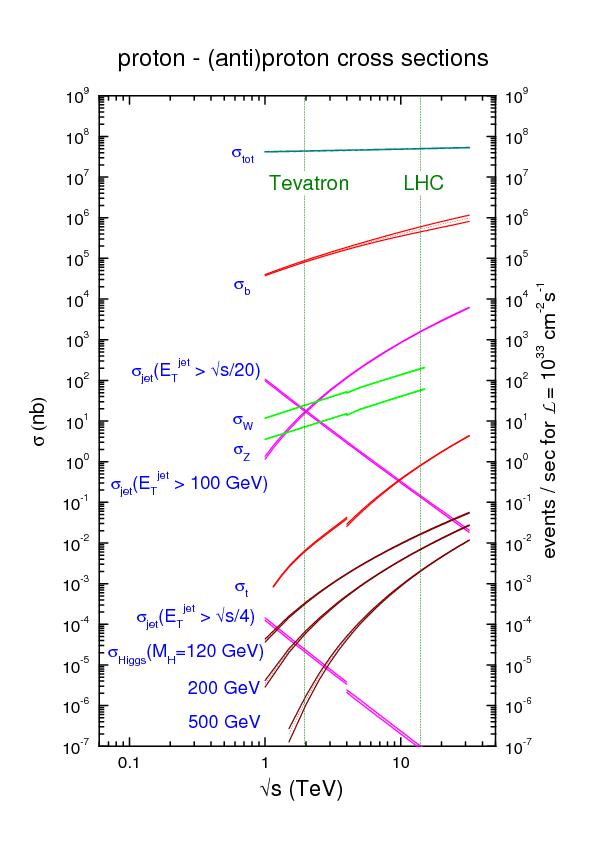
\includegraphics[width=3in]{figures/chapter2/cross_sec_plot.png}
    \caption{Standard Model production cross-section predictions at hadron-hadron colliders\cite{prod_crosssec}}
    \label{fig:crosssec}
\end{figure}

Another important characterization is luminosity, $\mathcal{L}$, which relates the production cross-section of a process to the observed production rate, $R$: $$R=\frac{dN}{dt}=\sigma\times\mathcal{L}$$ \noindent All modern colliders use bunched beams (described in additional detail in \ref{sec:acc_comp}). The luminosity of collider with two beams of bunch size $n_1$ and $n_2$ is expressed as $$\mathcal{L}=f_{coll}\frac{n_1n_2}{4\pi\sigma_x^*\sigma_y^*}.$$ \noindent Here, $\sigma_1^*$ and $\sigma_2^*$ describe the transverse beam size in the bend and vertical directions and $f_{coll}$ is the bunch crossing frequency of the collider. This luminosity equation relies on the assumptions that the bunches are identical in transverse profile, that the profiles are Gaussian and independent of position along the bunch, and the particle distributions are not altered during bunch crossing. Luminosity can be affected by non-zero beam crossing angles, $\Theta_C$, and bunch length $\sigma_z$. The luminosity will reduced by a factor $1/(1+\phi^2)^{1/2}$ where $\phi=\Theta_C\sigma_z/(2\sigma_x^*)$ \cite{pdg}. As with $E_{CM}$, maximizing luminosity is generally a goal of collider design. \\

%% SUBSEC: LHC
\subsection{The Large Hadron Collider}
The LHC is currently the world’s largest and most powerful particle accelerator. It is located at the European Organization for Nuclear Physics (CERN). Initial designs began in the 1980's, while CERN's previous collider, the Large Electron-Positron collider (LEP) was still under construction and taking data. The design was officially approved in 1994 and the first beams were circulated in 2008 \cite{lhc_guide}. CERN currently has 23 Member States, 7 associated Member States, and 6 Observer States, including the United States \cite{members}. These states, and many others with scientific contacts or cooperation agreements, finance and operate the LHC and receive access to the collected data. Thus, CERN continues to support its missions of strong international collaboration, scientific discovery, and technological innovation.\\

The LHC was constructed in the existing 27 km circular LEP tunnel under the French/Swiss border and consists of two parallel beampipes surrounded by magnets. It is used mainly to accelerate and collide protons, though other particles such as lead ions can be used for specific studies. The two beams run in opposite directions and intersect at four points along the ring where the detectors (ATLAS, CMS, ALICE, and LHCb) are located. The LHC magnet system consists of over 10,000 superconducting magnets including dipole magnets to guide the beams in a circular path, quadrupole magnets to focus the beams, and higher pole order magnets for small field corrections \cite{lhc_tdr}.\\

The initial plan for Run 1 of the LHC was to deliver data with $E_{CM}=\sqrt{s}=$14 TeV beginning in 2008. Unfortunately a week after initial beams were circulated in September 2008, a magnet quench occurred damaging 53 superconducting magnets and releasing approximately 6 tons of liquid helium. The projected timeline was adjusted, and physics data-taking began in 2009 at a reduced energy $\sqrt{s}=$7 TeV \cite{adj_commis}. The energy was increased to $\sqrt{s}=$8 TeV in 2012 and data taking continued until early 2013.\\

The LHC was shutdown from 2013-2015 to allow repairs and upgrades to the accelerator and detectors. Run 2 of the LHC began in 2015 at $\sqrt{s}=$13 TeV and continued until December 2019. During Run 2, the LHC delivered an integrated luminosity of 156$fb^{-1}$. Of this, 147 $fb^{-1}$ was recorded by ATLAS (the detector used in this thesis) and 139 $fb^{-1}$ passed quality requirements for use in physics analyses. A breakdown of the Run 2 luminosity, including luminosity delivered per year, is shown in Figure \ref{fig:run2_lumi}.\\

\begin{figure}[h]
    \begin{subfigure}
        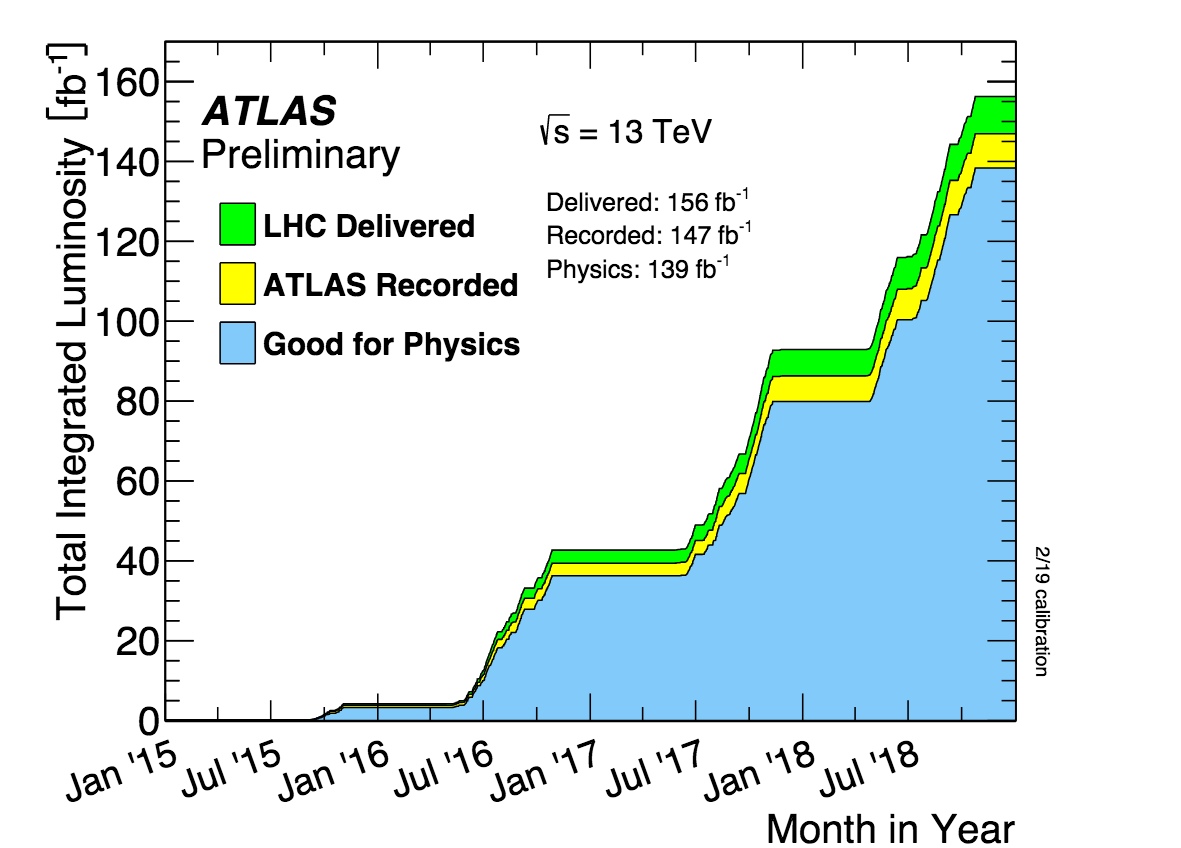
\includegraphics[width=3in]{figures/chapter2/run2_lumi.pdf}
    \end{subfigure}
    \begin{subfigure}
        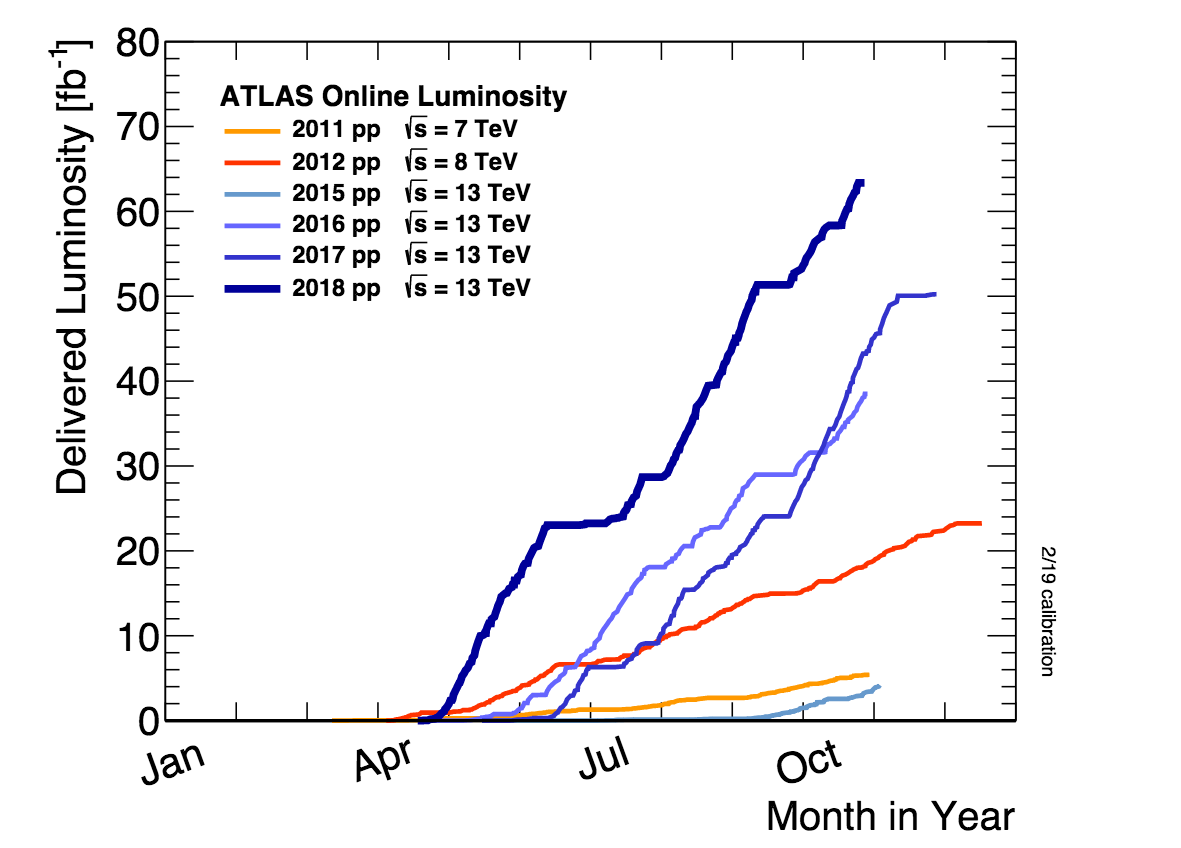
\includegraphics[width=3in]{figures/chapter2/run2_lumi_yrs.pdf}
    \end{subfigure}
    \caption{Left: total integrated luminosity delivered by the LHC (green), recorded by ATLAS (yellow) and usable for physics (blue). Right: Cumulative luminosity versus day delivered to ATLAS during stable beams and for high energy p-p collisions \cite{run2_lumi}.}
    \label{fig:run2_lumi}
\end{figure}

The LHC is currently in a second shutdown phase and Run 3 at $\sqrt{s}=$14 TeV is scheduled to begin in 2021. The tentative full-term schedule for the LHC is shown in Figure \ref{fig:schedule}, and the predicted luminosity growth in Figure \ref{fig:hl_lumi}. Run 3 is expected to continue until 2024, at which time a third shut-down will begin to allow commissioning of the High-Luminosity LHC (HL-LHC) which will proceed in three runs from 2026-2038 \cite{commissioning}.

\begin{figure}[htb!]
    \centering
    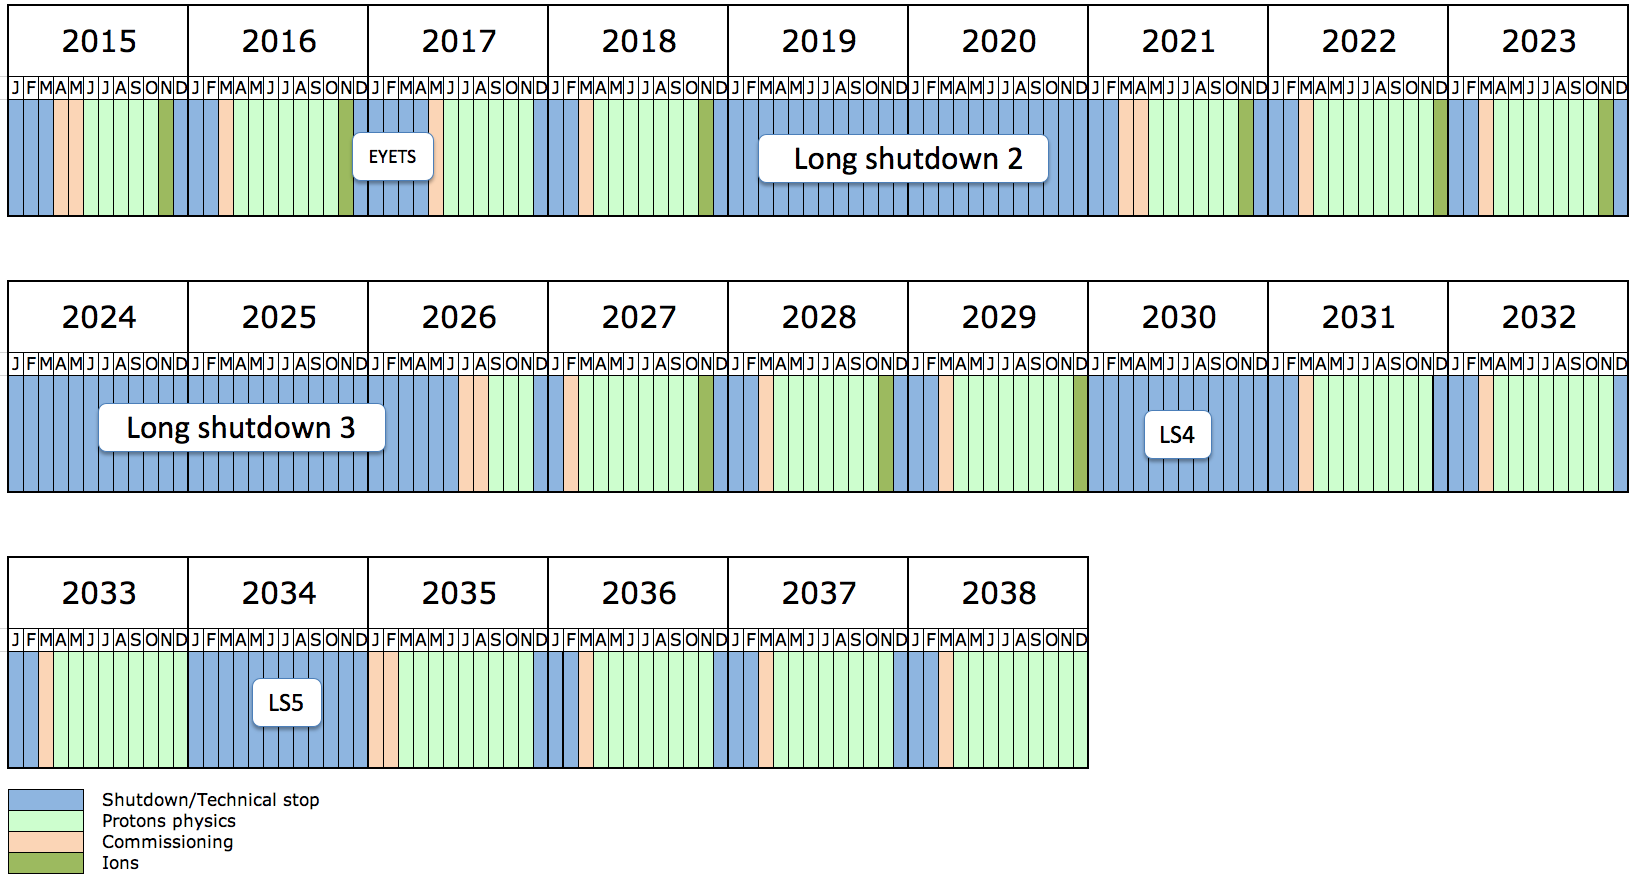
\includegraphics[width=4.5in]{figures/chapter2/lhc_sched.png}
    \caption{LHC planned operating schedule until 2038. EYETS stands for Extended Year End Technical Stop, a lengthened version of the annual brief shutdown during LHC running to allow for repairs. LS stands for Long Shutdown.}
    \label{fig:schedule}
\end{figure}

\begin{figure}[htb!]
    \centering
    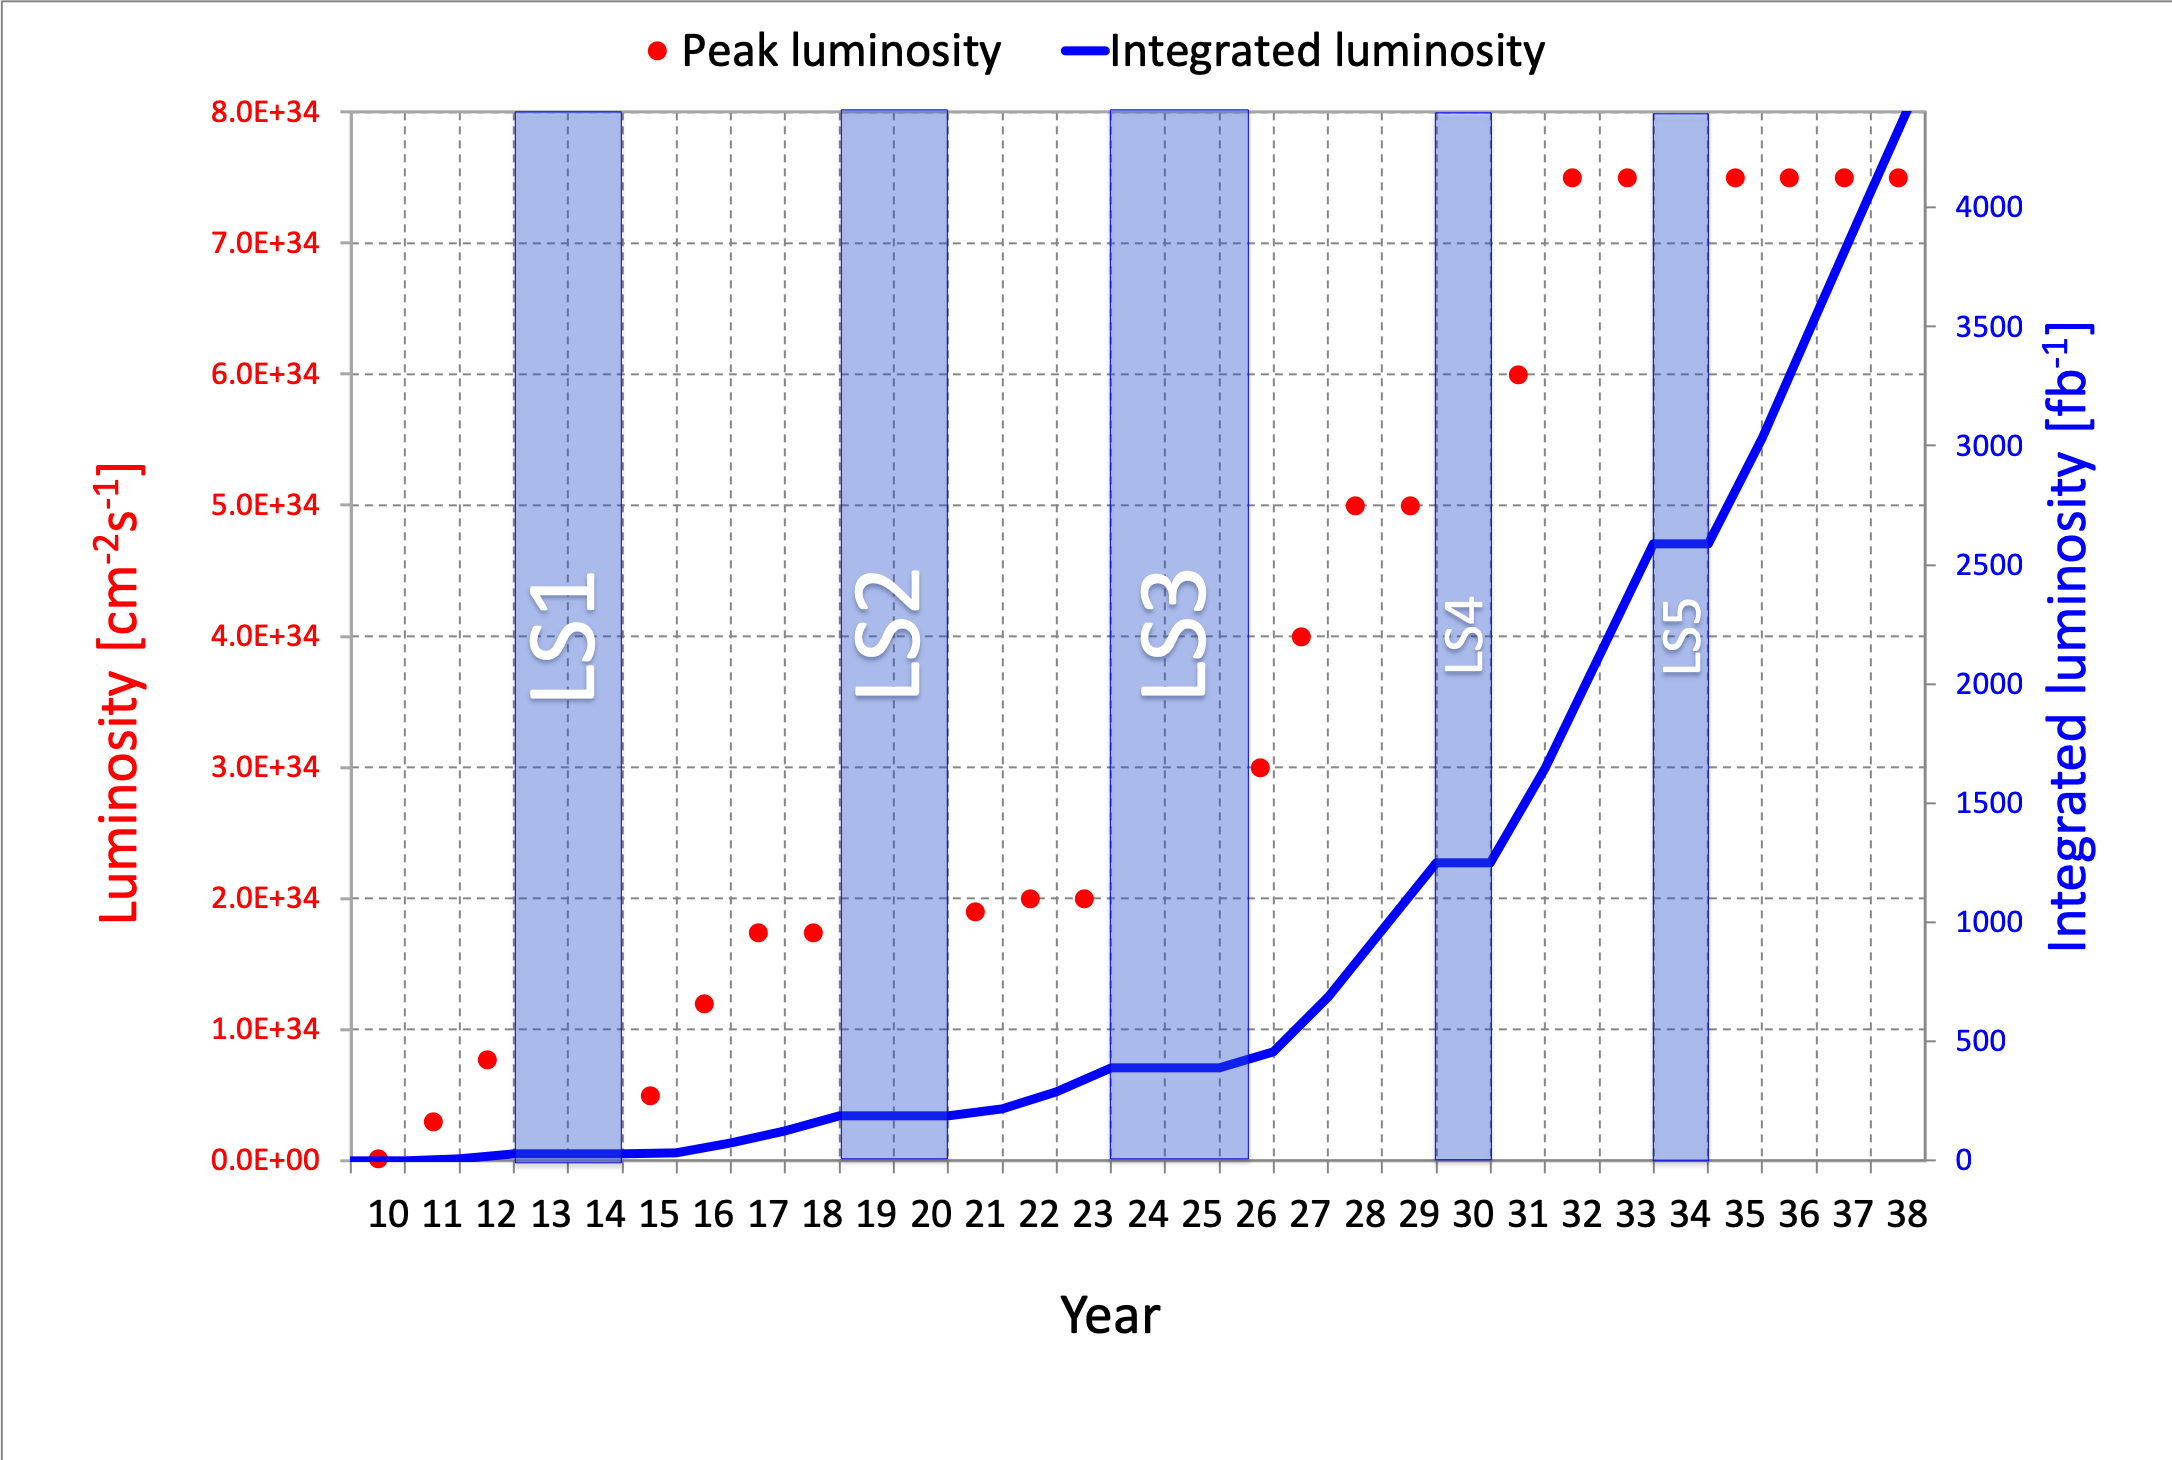
\includegraphics[width=3in]{figures/chapter2/hl_lumi.png}
    \caption{HL-LHC luminosity projection after completing Run 2}
    \label{fig:hl_lumi}
\end{figure}

%% SUBSEC: ACCELERATOR COMPLEX
\subsection{The LHC Accelerator Complex}\label{sec:acc_comp}
The LHC is supplied with high-energy protons through a multi-stage injector chain illustrated in Figure \ref{fig:acc_comp}. For proton-proton runs (as are used for this dissertation) hydrogen atoms from a concentrated source are passed through Linac2, a linear accelerator containing a strong electric field which removes the electrons from the atoms. This results in a pure proton beam with an energy of 50 MeV. This beam is then sent into the Proton Synchrotron Booster (PSB) which consists of 4 superimposed synchrotronic rings which further accelerate the beam to 1.4 GeV. The beam then enters the Proton Synchrotron (PS), a circular accelerator that increases the beam energy to 25 GeV. The PS feeds into the Super Proton Synchrotron (SPS), a 7km circular accelerator, where it reaches an energy of 450 GeV. Finally, the beam enters the main LHC ring where it is split into two beams that travel in opposite directions. Within the main ring the protons are grouped into bunches of approximately 115 billion protons each. This is a consequence of the oscillating frequency of the radio frequency cavities used to accelerate the protons and also allows collisions to occur at discrete intervals. Within the main ring, protons are further accelerated to their maximum energy of 6.5 TeV (in Run 2) and then circulate within the ring for several hours as collisions occur at the interaction points \cite{lhc_guide}.\\

\begin{figure}[h]
    \centering
    \includegraphics[width=5in]{figures/chapter2/acc_complex.png}
    \caption{The CERN Accelerator Complex}
    \label{fig:acc_comp}
\end{figure}

The protons in the LHC circulate in a defined and discrete bunch structure. During normal operation, bunches of roughly $10^{11}$ protons are separated by 25 nanosecond gaps, and a full LHC ring holds 2808 bunches. The bunches begin on the order of a few centimeters in size and are compressed to around 20 $\mu$m near the interaction points to increase the potential for collisions. This bunch structure allows for an interaction frequency of 40 MHz; however, to provide ramp up time for beam injection or magnet quenching, the actual interaction frequency is closer to 30 MHz \cite{lhc_machine}.\\

During bunch crossings, the interaction of interest is the hard-scattering collision where the quarks within the colliding protons transfer large amounts of momentum resulting in a system of large mass \cite{hard_scattering}. Although it is rare for more than one hard-scattering event to occur in a single bunch crossing, multiple soft interactions are expected. The particles resulting from these soft interactions overlap with particles from the hard-scattering event, a phenomena referred to as pileup. LHC analyses distinguish between two types of pileup: instantaneous, which involves particles from the same bunch crossing, and out-of-time, which involves particles from previous or following bunch crossings. Both types of pileup contribute to crowding in the detectors and complicate particle reconstruction \cite{pileup}. The average pileup for Run 2 is shown in Figure \ref{fig:pu}.\\

\begin{figure}[h]
    \centering
    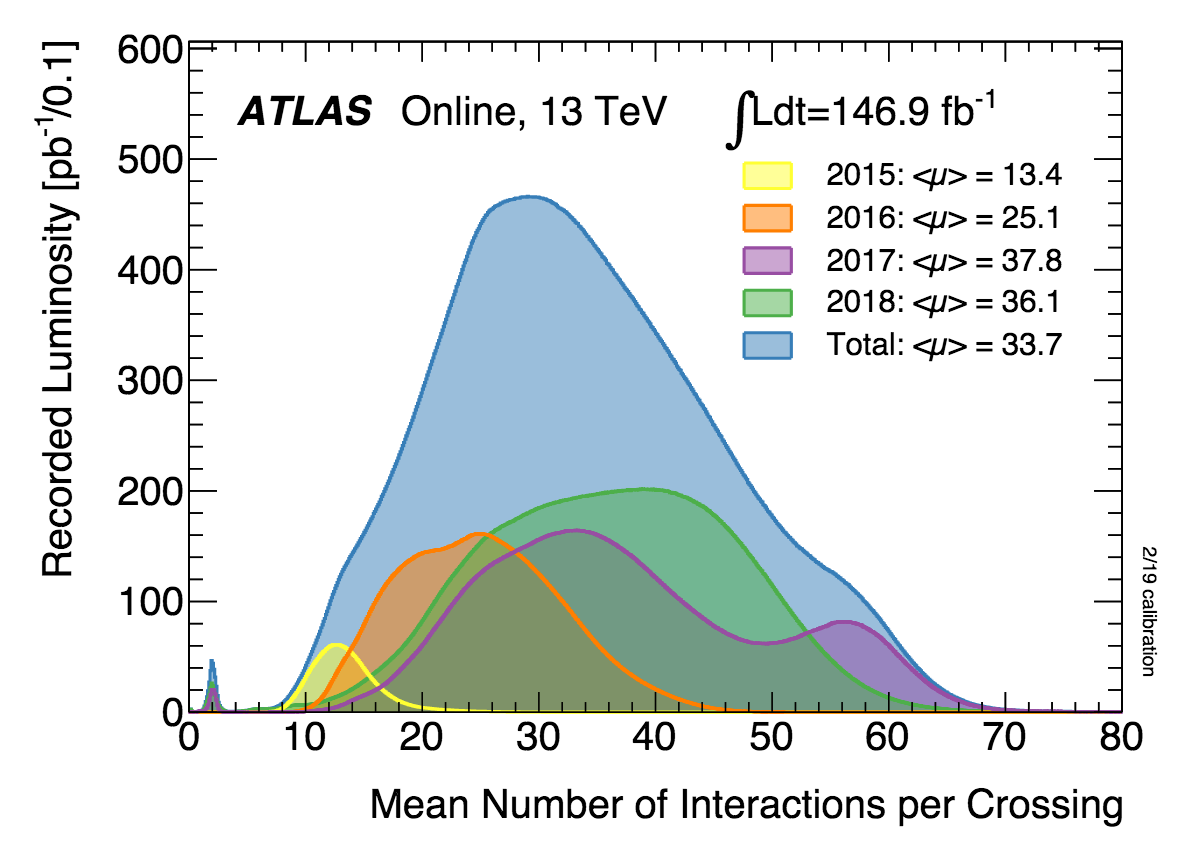
\includegraphics[width=3.5in]{figures/chapter2/run2_pu.pdf}
    \caption{The luminosity-weighted distribution of the mean number of interactions per crossing for the Run 2 pp collision data at 13 TeV center-of-mass energy \cite{run2_lumi}}
    \label{fig:pu}
\end{figure}


%%SECTION: DETECTORS
\section{Particle Detection}

After the initial hard-scattering event a variety of particles are produced either as direct products of the collision or as decays of the initial particles. Detectors at the interaction points aim to measure these particles. Only particles which have a long enough lifetime and interact with SM particles are detectable. However after reconstructing these particles (as described in Chapter 3), imposing additional constraints such as momentum and energy conservation, and accounting for inefficiencies in the detector, physicists can find evidence for other particles such as neutrinos or BSM particles that likely occurred before or alongside the detected particles.\\

Modern detectors at collider facilities rely on two primary technologies. Semiconductor detectors use materials such as silicon to create diodes and charged particles passing through the material create currents that can be tracked and measured. Calorimeters are typically designed to absorb particles and use scintillating materials to measure the resulting energy showers. Additional common methods of particle detection include Transition Radiation counters or Cherenkov Light measurements \cite{detector_physics}.

%%%SUBSEC: ATLAS
\subsection{The ATLAS Detector}
ATLAS (A Torroidal LHC ApparatuS) is one of the two general physics detectors at the LHC (along with CMS) and was designed to effectively detect various SM particles for refined SM measurements and new physics searches. It is one of the largest particle detector ever built at 46m long, 25m in diameter, and it weighs over 7,000 tons \cite{tdr1}\cite{tdr2}. \\

A schematic of the detector is shown in Figure \ref{fig:atlas_schem}. ATLAS consists of 4 subsystems (described below) which wrap concentrically around the beamline. The detector can be divided into two geometric components: the barrel, which wraps around the beamline, and the endcaps which are perpendicular to the beamline at either end of the detector.\\

\begin{figure}[h]
    \centering
    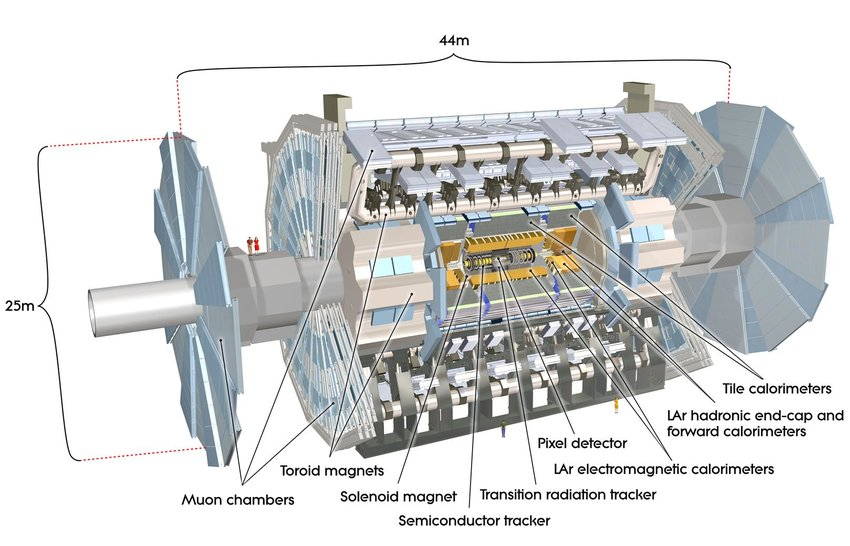
\includegraphics[width=4.5in]{figures/chapter2/atlas_schem.png}
    \caption{Diagram of the various subsystems of the ATLAS detector \cite{atlas}}
    \label{fig:atlas_schem}
\end{figure}

A right-handed coordinate system is used to describe position within ATLAS. The origin of the coordinate system is set to be the event interaction point; from this origin the beam defines the $\hat{z}$ direction and the $\hat{x}\text{-}\hat{y}$ plane is perpendicular to the beamline. The positive $\hat{x}$ direction is towards the center of the LHC ring and the positive $\hat{y}$ direction is straight up. Vector components in the $\hat{x}\text {-}\hat{y}$ plane are called transverse. Transverse components are particularly important in physics analyses because they are invariant to boosts in the $\hat{z}$ direction that come from particles' initial velocities.\\

The cylindrical symmetry of the detector allows for the definition of additional angular coordinates. The azimuthal angle $\phi$ is measured around the beam axis and is zero towards the center of the LHC ring.  The polar angle $\theta$ is the angle from the beam axis and is zero along the beamline. A common reparameterization of the polar angle is the pseudo-rapidity $\eta=-\text{ln(tan(}\theta/2))$. Particles along the beamline thus have a pseudo-rapidity $\eta=\infty$ and particles perpendicular to it have pseudo-rapidity $\eta=0$. For massive particles, the standard rapidity $y=1/2\text{ln[(E}+p_Z)/(\text{E}-p_Z)]$ can also be used. Angular distances in the $\eta\text{-}\phi$ plane are described by $\Delta\text{R}=\sqrt{\Delta\eta^2+\Delta\phi^2}$ \cite{atlas}.\\

Finally, the centrality of objects within a detector can be described in terms of impact parameters. The impact parameter $d_0$ is the signed distance from a charged track to the z axis while $z_0$ is the z-coordinate of the track at the point of closest approach to the global z axis (Figure \ref{fig:impac_params}). These parameters are calculated during track fitting as described in Chapter 3.

\begin{figure}[h]
    \centering
    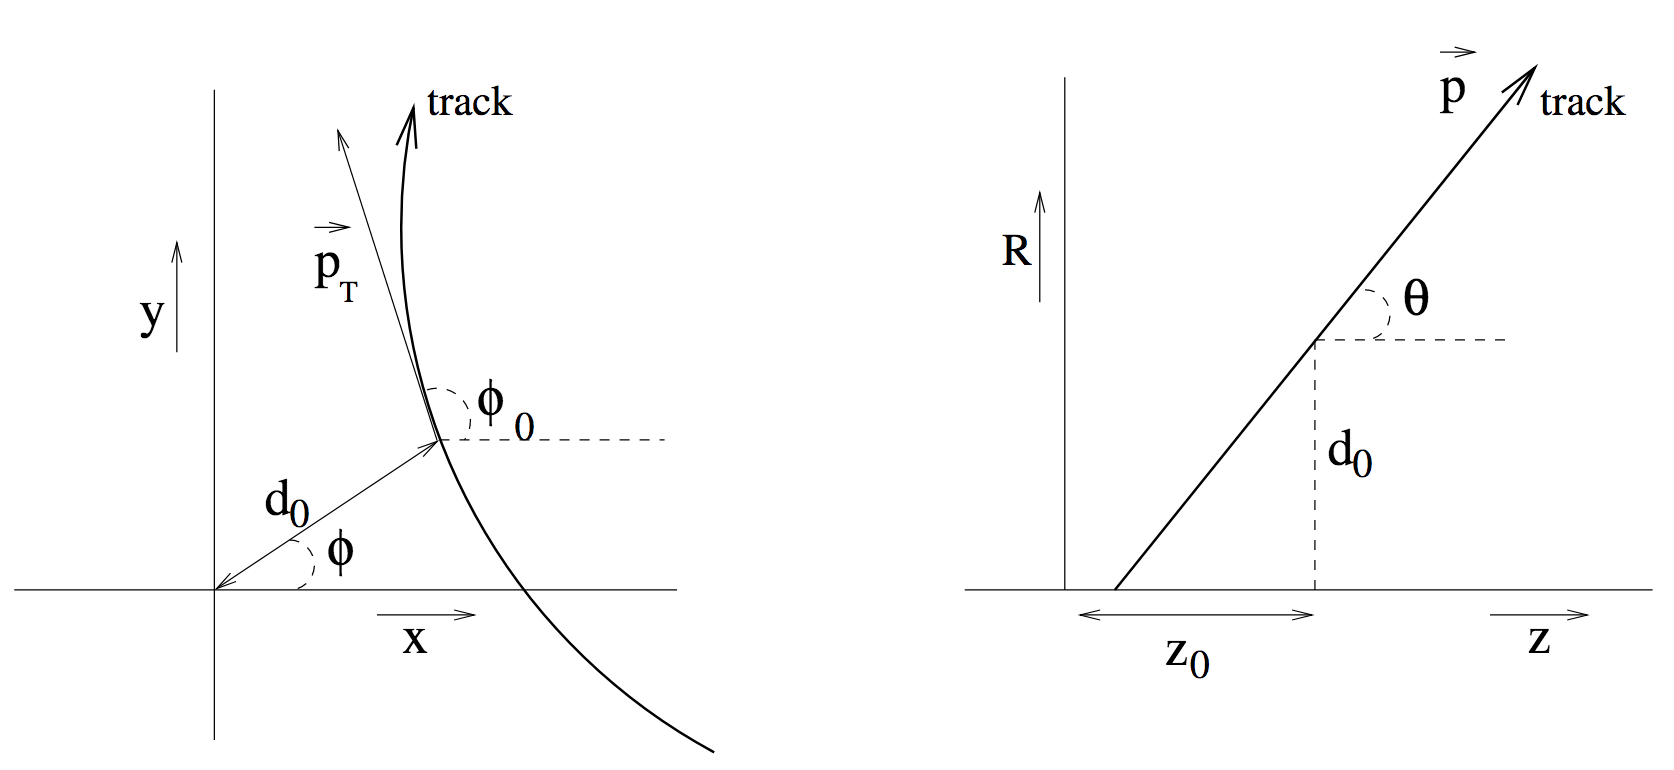
\includegraphics[width=3.5in]{figures/chapter2/impact_params.png}
    \caption{Illustration of impact parameters in the transverse plane (left) and R-Z plane (right).}
    \label{fig:impac_params}
\end{figure}

%%% INNER DETECTOR
\subsubsection{Inner Detector}
The Inner Detector is closest to the interaction point and consequently is highly sensitive and compact. It is designed to allow for robust track-finding algorithms, precise momentum resolution, and accurate vertex reconstruction. The Inner Detector, shown in Figure \ref{fig:id}, consists of 3 specialized, high granularity detectors (all surrounded by a 2T magnetic field) that measure the momentum, direction, and charge of charged particles. It provides full coverage in $\phi$ for $|\eta|<2.5$ \cite{inner_detec}.\\

The innermost portion of the Inner Detector is the Pixel Detector. It is the highest granularity subsystem of the Inner Detector and includes 4 concentric cylindrical layers around the beamline and 3 parallel layers in each endcap. Each layer consists of 10 $\text{cm}^2$ modules of 46,080 silicon pixels, each with its own readout channel. This corresponds to a position resolution of 14 x 115 $\mu\text{m}^2$ and allows for high definition track reconstruction with up to 4 hits per track (described further in Chapter 3) near the interaction point, yielding precise impact parameter reconstruction. The innermost cylindrical layer, called the Insertable B-Layer (IBL), was added for Run 2 to mitigate radiation damage suffered in Run 1 \cite{ibl}.\\

\begin{figure}[h]
    \centering
    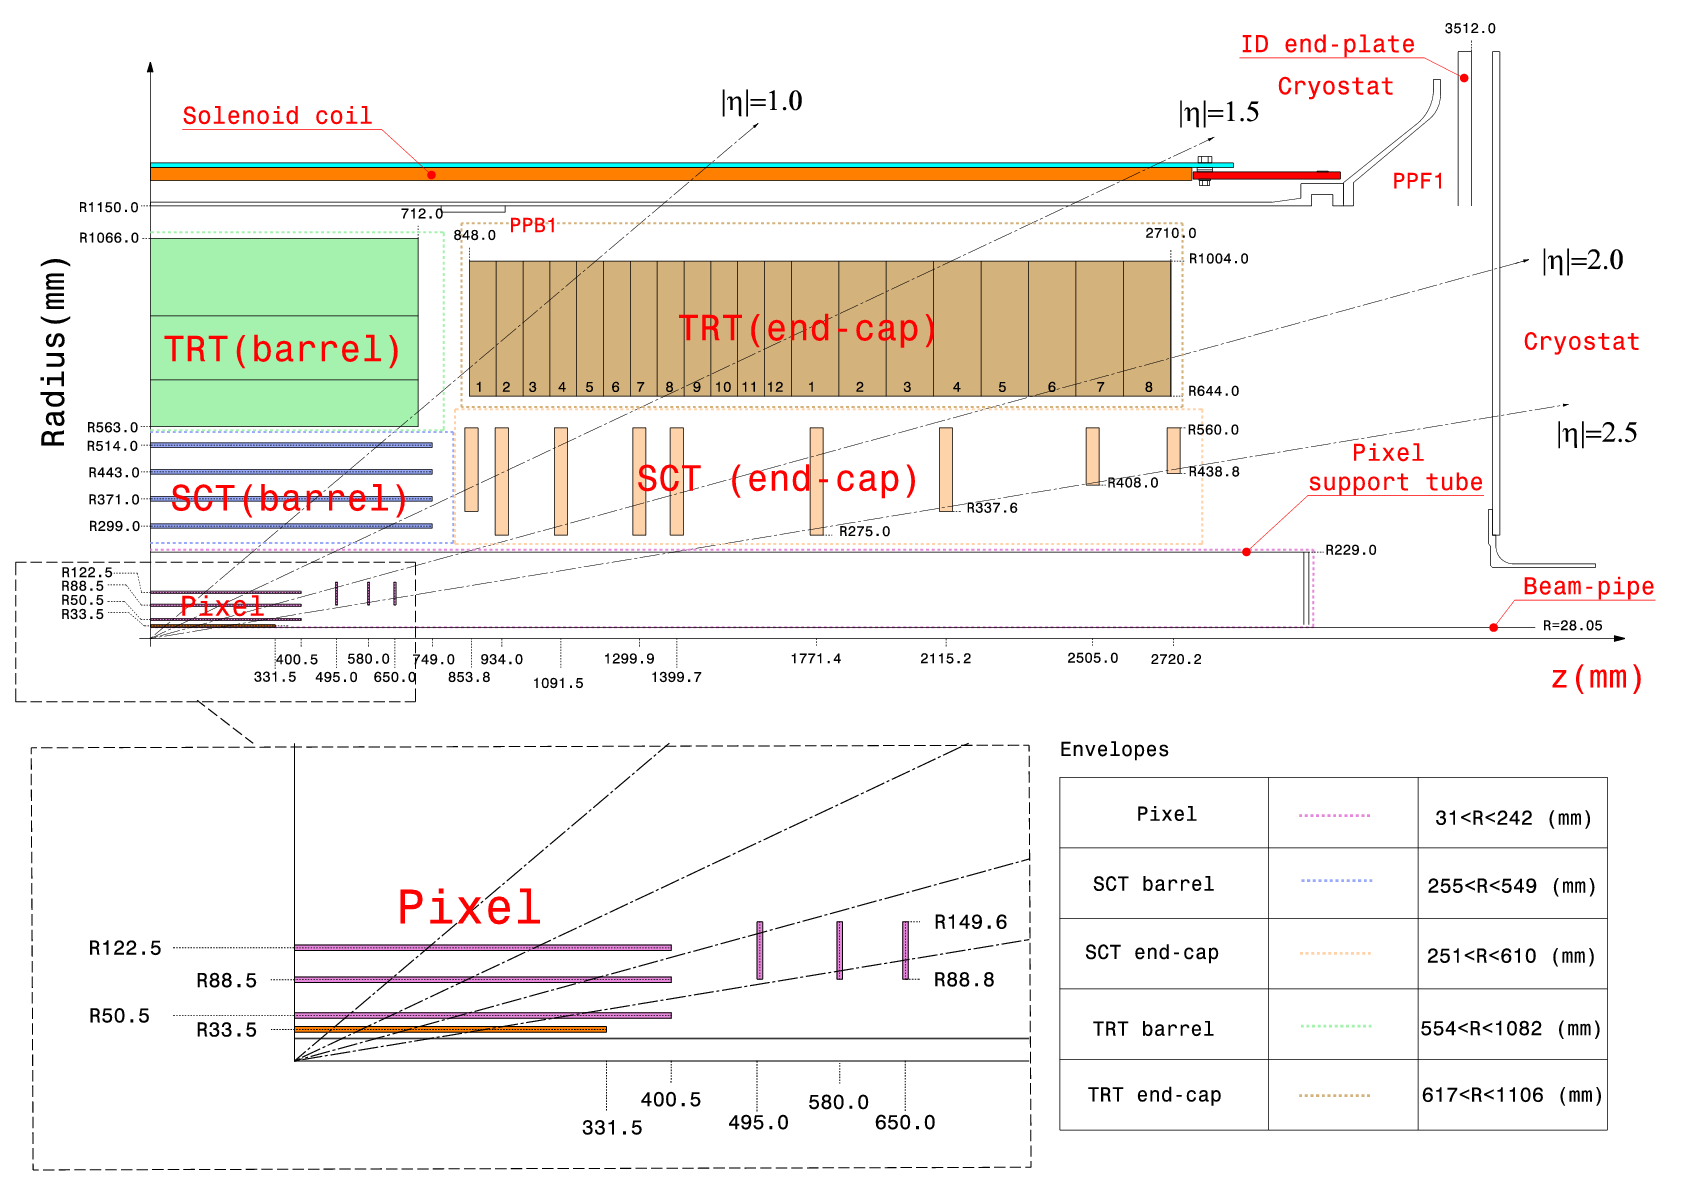
\includegraphics[width=5in]{figures/chapter2/inner_detec.png}
    \caption{The $r\text{-}z$ cross-section of one quandrant of the ATLAS Inner Detector. The top figure is the whole inner detector and the lower figure is a magnified view of only the pixel detector \cite{inner_detec}.}
    \label{fig:id}
\end{figure}

The semiconductor tracker (SCT) is silicon microstrip detector with 4088 double sided modules distributed between 4 barrel layers and 9 endcap layers. There is a readout component every 80 $\mu$m providing a resolution of 17 $\mu$m. This allows up to 8 precision hits per track which contributes to improved momentum measurement and vertex reconstruction. In both the Pixel Detector and SCT, hits are defined as electron-hole drifts in the applied electric field resulting from electrons freed from orbit by incident particles.\\

Finally, the Transition Radiation Detector (TRT) is made of 4mm diameter gas-filled drift-tube straws interleaved with radiators (fibers in the barrel and foils in the endcaps). There are 50,000 straws in the barrel and 250,000 straws in the endcaps, each end of each straw is read out separately, allowing a position resolution of 0.17 mm. In addition to providing continuous tracking, the TRT improves the identification of charged particles like electrons and pions. The fibers and foils have different dielectric constants than the straws, and when charged particles pass through the boundaries, transition radiation photons are produced. The amount of transition radiation produced corresponds inversely to the incident particle's mass. Each straw readout provides two independent thresholds to distinguish tracking hits (lower threshold) from transition radiation hits (higher threshold) \cite{trt}.


%%% CALOS
\subsubsection{Calorimeters}
Calorimeters measure the energy of particles by absorbing them. ATLAS has two sampling calorimeter subsystems, shown in Figure  \ref{fig:calos}, which absorb particles and electronically sample the resulting energy shower distributions. Together these calorimeters cover the range $|\eta|<4.9$; the $|\eta|$ region matched to the inner detector has a finer granularity for precision measurements of charged particles, while the extended $|\eta|$ range has a coarser granularity suitable for hadronic jet reconstruction \cite{atlas}.\\

\begin{figure}[htb!]
    \centering
    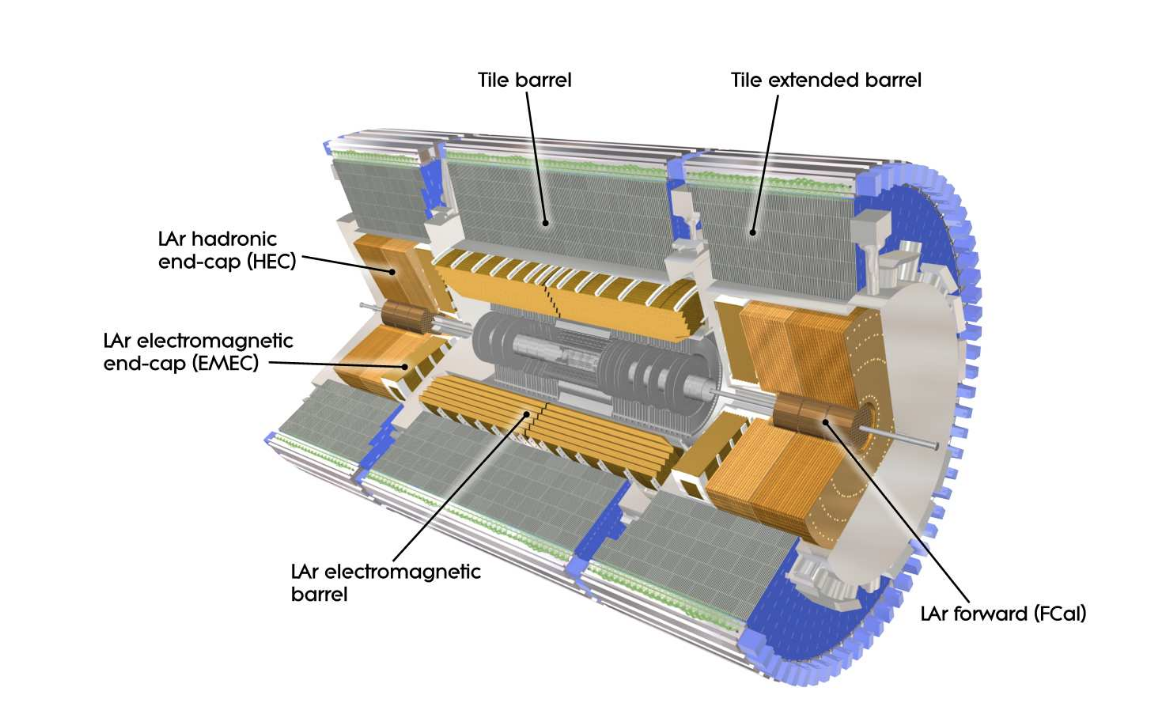
\includegraphics[width=4in]{figures/chapter2/calos.png}
    \caption{Cut-away view of the ATLAS calorimeter system \cite{atlas}}
    \label{fig:calos}
\end{figure}

The electro-magnetic (EM) calorimeter is designed to absorb and measure charged particles, mainly electrons and photons. It consists of a barrel component covering $|\eta|<1.5$ and two endcaps covering $1.4<|\eta|<3.2$. The barrel and endcaps contain 3 layers of accordion shaped lead plates which are separated by layers of liquid argon (LAr) and readout electrodes (Figure \ref{fig:em_calo}). The accordion structure allows full azimuthal coverage with no cracks \cite{em_calo_run2}.\\

\begin{figure}[htb!]
    \centering
    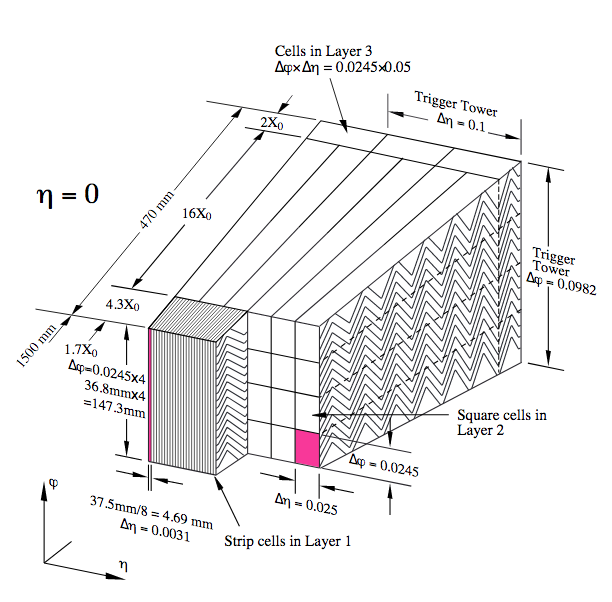
\includegraphics[width=3.5in]{figures/chapter2/em_calo.png}
    \caption{The accordion geometry used in the EM calorimeter \cite{em_calo_run2}.}
    \label{fig:em_calo}
\end{figure}

\pagebreak

As charged particles move through the EM calorimeter, their interactions with the lead absorbers create showers of charged particles through bremmstrahlung radiation and electron-positron pair production. These particle showers then ionize the liquid argon and an applied high-voltage in the LAr filled gap guides the resulting ions and electrons to the readout electrodes. This process can repeat in multiple layers of the calorimeter with each successive shower having decreased energy \cite{em_calo_run2}. The types and amounts of materials used in the EM calorimeter determine its radiation length, $X_0$, which is defined as the average distance an electron can travel before its energy is reduced by a factor $1/e$. The radiation length is given in terms of atomic weight $A$ and atomic number $Z$ as $X_0=\frac{716.4 A}{Z(Z+1)\text{ln}(287/\sqrt{Z})}$ \cite{pdg}. Lead is a high-Z material and hence allows for a small radiation length.\\

The first layer of the EM calorimeter extends to a depth of 4.3$X_0$ and consists of strip towers segmented in $\eta$. The strips are finely segmented (ie 8 strips in front of a central cell) in the central $\eta$ region ($|\eta|<1.4$) and become coarser as $\eta$ increases. The full calorimeter granularity is described in Table \ref{tab:calos}. The second layer is made of square towers of size $\eta \times \phi=0.025\times0.025$ for $|\eta|<2.5$ and size $\eta \times \phi = 0.1 \times 0.1$ for $|\eta|>2.5$. The second layer extends to a depth of 16$X_0$. The third layer covers only $|\eta|<2.5$ with towers of size $\eta \times \phi = 0.05 \times 0.025$ and extends to a depth of 2$X_0$. Additionally, for $|\eta|<1.8$, there is a presampler consisting of an active LAr layer to correct for energy lost upstream in the calorimeter \cite{atlas}. Collectively, these layers provide sufficient material to absorb nearly all electrons and photons. A summary of the absorption material in all calorimeters is shown in Figure \ref{fig:int_lens}.\\

\begin{figure}[htb!]
    \centering
    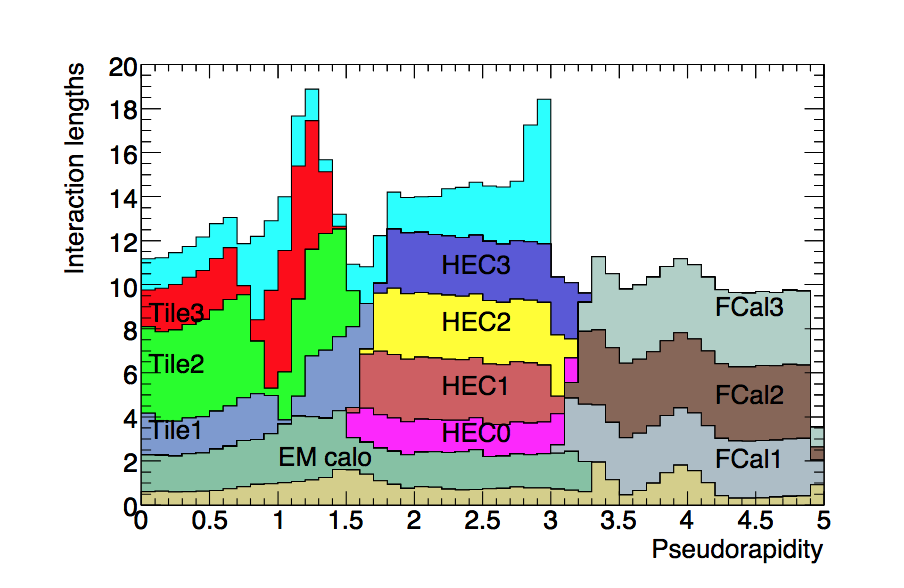
\includegraphics[width=3.5in]{figures/chapter2/calo_int_lens.png}
    \caption{Cummulative amount of material, in units of interaction length, for different components of the ATLAS calorimeter. Tile$_i$ refers to layers of the TileCal, HEC$_i$ refers to layers of the Hadronic End Caps, and FCal$_i$ refers to layers of the Forward Calorimeter \cite{atlas}.}
    \label{fig:int_lens}
\end{figure}

\begin{table}
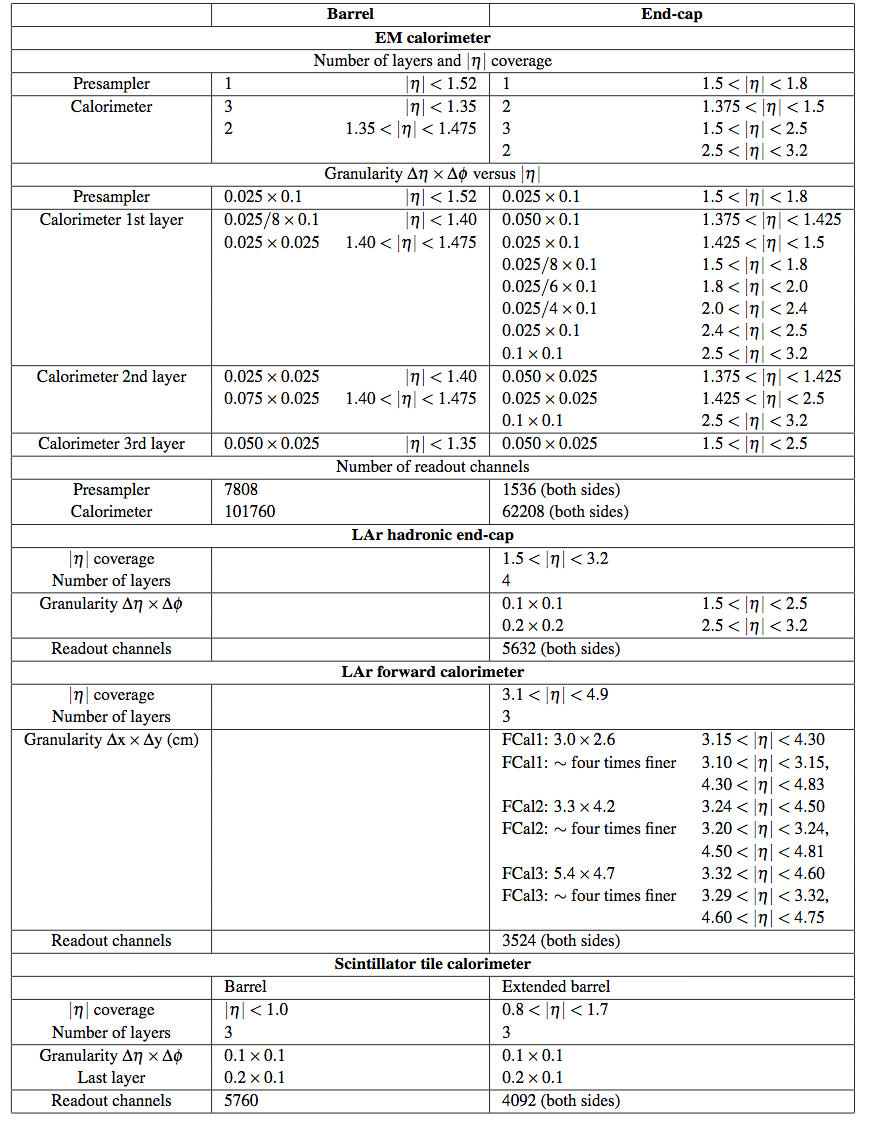
\includegraphics[width=5.5in]{figures/chapter2/calo_gran.png}
    \caption{Coverage, granularity, and number of readout channels of the ATLAS calorimeter system \cite{atlas}.}
    \label{tab:calos}
\end{table}

The hadronic calorimeters are positioned outside the EM calorimeters and consist of a central barrel in the region $|\eta|<1.0$, two extended barrels in the regions $0.8<|\eta|<1.7$, and two endcaps in the region $1.5<|\eta|<3.2$ \cite{atlas}. The granularity of these components are described in Table \ref{tab:calos}. The hadronic calorimeters are used to absorb and record showers of hadronic particles which interact via the strong force.\\

The central and extended barrels are collectively referred to as the Tile Calorimeter (TileCal), and consist of scintillating tiles separated by steel plates. Hadronic showers begin in the EM calorimeter where strong interactions with the argon and lead nuclei produce additional hadrons, and this process continues into the TileCal; some particles in hadronic showers may also interact electromagnetically.\\

Each cylinder in the TileCal contains 64 modules, and the tiles in each module are placed in the plane perpendicular to the beamline and staggered in depth (Figure \ref{fig:had_calo}). Similar to the EM calorimeter, charged particle interactions in the scintillating tiles create an electronic signal. This signal is read out by wave length shifting fibers on either end of the module and sent to photomultiplier tubes (PMTs). Each tile is readout by two PMTs \cite{tilecal}.\\ 

\begin{figure}[h]
    \centering
    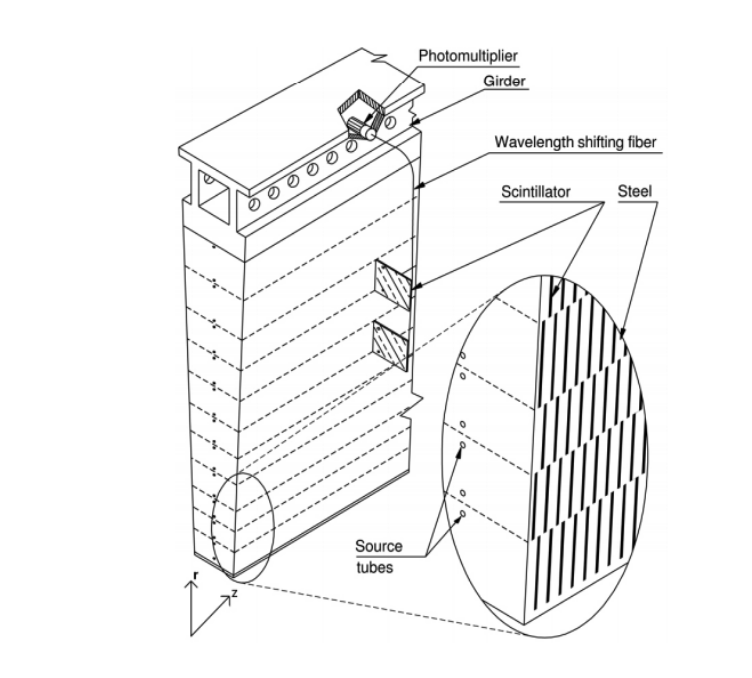
\includegraphics[width=3in]{figures/chapter2/had_calo.png}
    \caption{Schematic diagram of a $\phi$ wedge of the Tile Calorimeter \cite{tilecal}.}
    \label{fig:had_calo}
\end{figure}

The depth of hadronic calorimeters is characterized by the nuclear interaction length, $\lambda$, which describes the mean distance travelled by a hadronic particle before undergoing an inelastic nuclear interaction. The 4.7 to 1 ratio of steel to scintillator in the TileCal creates a nuclear interaction length of $\lambda$=20.7 cm. The EM calorimeter provides nearly 2$\lambda$ of material and the hadronic calorimeter provides over 8$\lambda$ altogether.\\ 

The hadronic endcaps function similarly to the EM calorimeter. They consist of flat copper plates separated by LAr and are segmented into four longitudinal layers \cite{em_calo_run2}. The granularity is described in Table \ref{tab:calos}.\\

Additionally, ATLAS contains a foward hadronic calorimeter (FCAL) covering $3.1<|\eta|<4.9$. The FCAL consists of 3 longitudinal layers in which cylindrical LAr gaps are arranged in matrices of copper (first layer) or tungsten (second and third layers) with electrod readouts. The FCAL is used for reconstruction of forward jets and operation in high pile-up environments \cite{em_calo_run2}.\\ 

%%% MUONS
\subsubsection{Muon Spectrometer}
Muons are minimally ionizing particles which allows them to often pass through the calorimeters with limited interaction. The Muon Spectrometer is the outermost subsystem of ATLAS and was designed to capture muons that have punched through the calorimeters and to provide standalone muon reconstruction, momentum measurement, and triggers. The muon spectrometer is shown in Figure \ref{fig:muon_sys} and consists of three concentric cylinders in the barrel region ($|\eta|<1$) and four end cap disks on either side ($1<|\eta|<2.7)$\cite{muon_tdr}.\\

\begin{figure}[h]
    \centering
    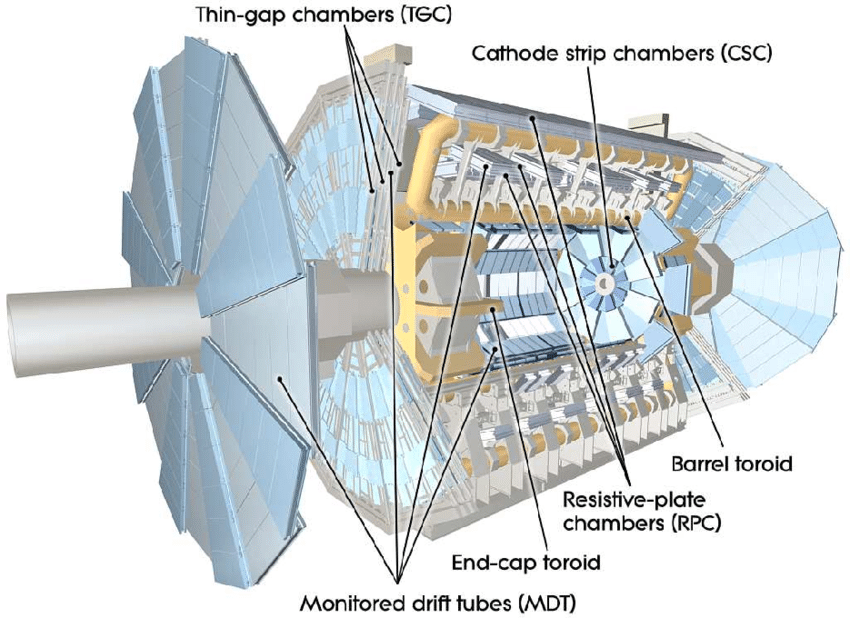
\includegraphics[width=4in]{figures/chapter2/muon_sys.png}
    \caption{Cut-away view of the ATLAS muon system \cite{atlas}.}
    \label{fig:muon_sys}
\end{figure}

Over most of the $|\eta|$ range, muon track coordinates are measured by Monitored Drift Tubes (MDTs). Charged particles passing through the MDTs will ionize gas atoms within the tubes and these ions will then drift and be readout by a tungsten anode wire. The MDT system consists of 1,171 chambers and 354,240 individual tubes which provide a resolution of 80 $\mu$m. At larger pseudorapidities ($2<|\eta|<2.7$) fine-granularity Cathode Strip Chambers (CSCs) are used in the first layer of the muon spectrometer to provide additional discriminating power in high occupancy environments. The CSCs are segmented in $\phi$ in 8 chambers and each chamber consists of an anode wire oriented in the radial direction with multiple cathode strips laid perpendicularly across. Crossing muons will deposit charges on multiple strips and interpolating between these chargers provides a position measurement. The CSCs provide a resolution of 60 $\mu$m \cite{muon_tdr}.\\

The muon trigger system covers the range $|\eta|<2.4$ and supports precise momentum measurements and track information orthogonal to that provided by the MDTs and CSCs. In the barrel, two layers of Resistive Plate Chambers (RPCs) are assembled with the middle layer of the MDTs and a third layer of RPCs is placed outside the final MDT layer (Figure \ref{fig:muon_schem}). RPCs consist of a small gas-gap between two parallel resistive plates; charged particles passing the gas-gap will create a shower of electrons that drift to the readout anode. Each RPC unit contains two gas-gaps, one oriented in the $\phi$ direction and the other in the $\eta$ direction. In the endcaps, three layers of Thin Gap Chambers (TGCs) are positioned perpendicular to the beam axis. TGCs are multi-wire proportional chambers; the wires are held at high-voltage and connected to grounded cathode planes which collect ionization charges. The high voltage and close proximity of the wires in the TGCs allows excellent time resolution \cite{muon_tdr}.\\ 

\begin{figure}[h]
    \centering
    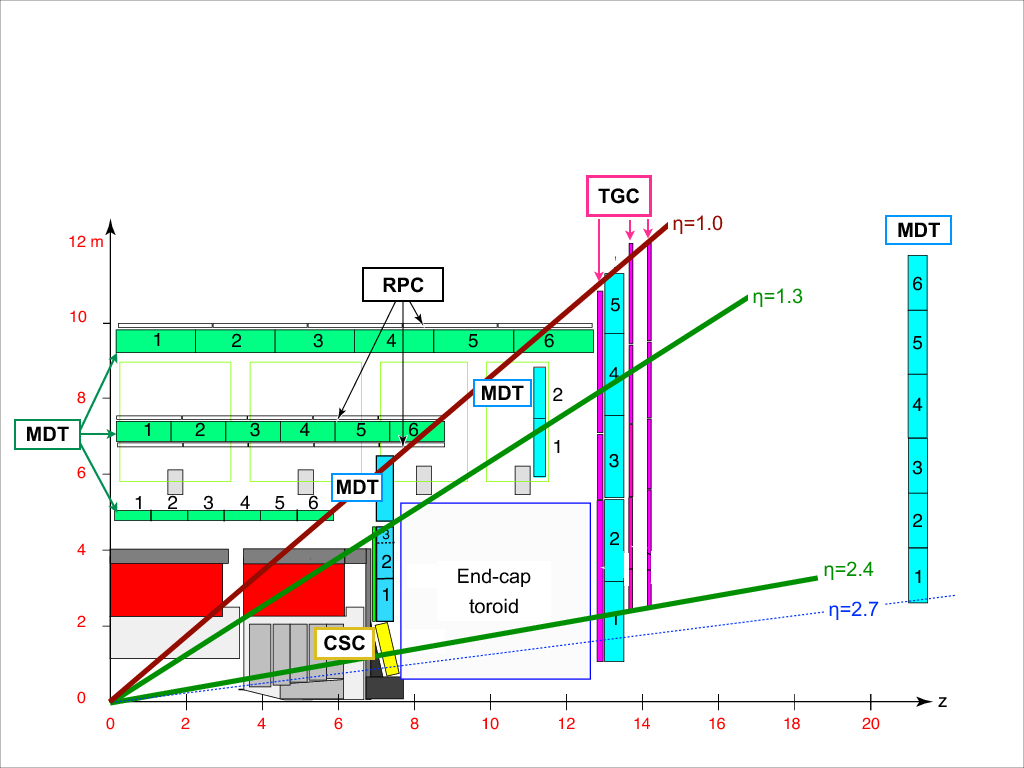
\includegraphics[width=4in]{figures/chapter2/muon_schem.png}
    \caption{A schematic picture showing a quarter-section of the muon system in a plane containing the beam axis \cite{muon_run2}.}
    \label{fig:muon_schem}
\end{figure}

%%% MAGNET SYSTEM
\subsubsection{Magnet System}
The ATLAS Magnet System bends the tracks of charged particles to allow momentum measurements. The track bending is caused by the Lorentz force:  $\textbf{F}=q\textbf{E}+q(\textbf{v}\times\textbf{B})$ and is hence proporitional to the particle's velocity. The magnet system is shown in Figure \ref{fig:magnets}. It has three components: a 2T solenoid magnet encompassing the inner detector, a 0.5T torroid in the barrel region of the muon spectrometer, and 2 1T torroids in each of the muon spectrometer endcaps \cite{magnet_tdr}.\\

\begin{figure}[h]
    \centering
    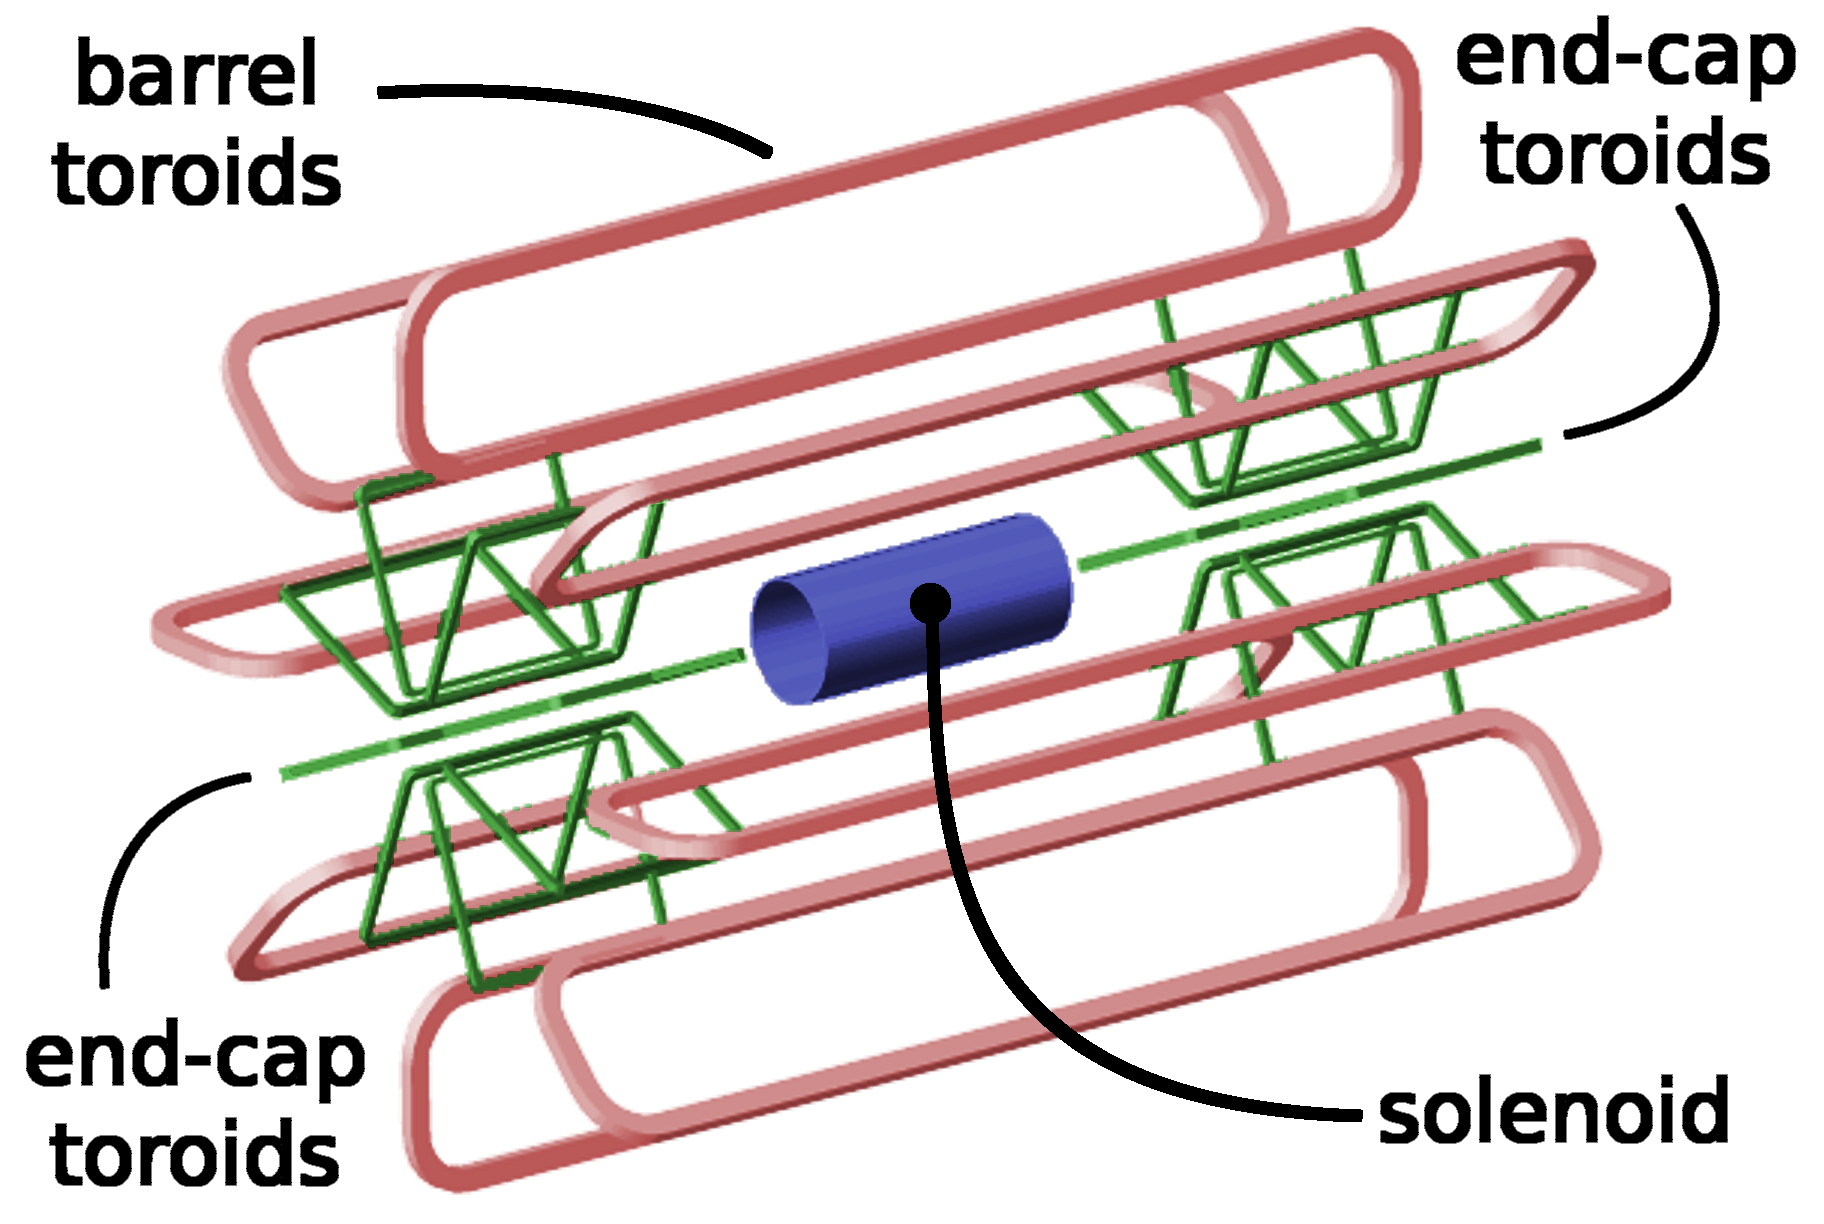
\includegraphics[width=3in]{figures/chapter2/magnets.png}
    \caption{Schematic diagram of the ATLAS magnet system}
    \label{fig:magnets}
\end{figure}

The central solenoid is a conduction cooled superconducting solenoid with minimum radial thickness. The barrel and endcap toroids each contain 8 air-core superconducting coils. These unique toroid magnets are what gives the ATLAS detector its name.